\chapter{On Reasoning, Memory, and Planning of Language Agents}
\label{chap:lec03_reasoning_memory_planning}
\section{本讲学习目标}

第三讲的任务不是再介绍一个局部 prompting trick，而是为整门课提出一个更宽的对象：\textbf{language agents}。Yu Su 的观点是，当前这波 agent 之所以值得重新讨论，不是因为它们能说更多话，而是因为语言本身正在变成一种用于\textbf{推理（reasoning）、记忆组织（memory organization）、规划（planning）和多模块协调}的通用表示层。

读完本讲后，读者应能回答：
\begin{itemize}
\item 为什么 Yu Su 主张使用 “language agent” 这个术语，而不是把一切都塞进笼统的 AI agent 桶里。
\item 为什么当前 RAG 还不足以支撑长期记忆，HippoRAG 试图补什么。
\item 什么叫 implicit reasoning，为什么 Grokked Transformers 说明“没有显式 CoT 不等于没有推理”。
\item WebDreamer 为什么代表了 language-agent planning 从 reactive execution 走向 model-based planning 的关键转折。
\item memory、reasoning 和 planning 为什么必须一起设计，而不能孤立优化。
\end{itemize}

\section{背景与统一框架}

\subsection{为什么又是 agents}

Yu Su 用经典定义重新开场：agent 是能够通过传感器感知环境、并通过执行器对环境施加动作的系统。把这一定义代入当代 LLM，就会立刻发现一个变化：模型不再只处理纯文本输入输出，而是位于感知、动作、反思与环境反馈之间的闭环中。

\begin{figure}[H]
\centering
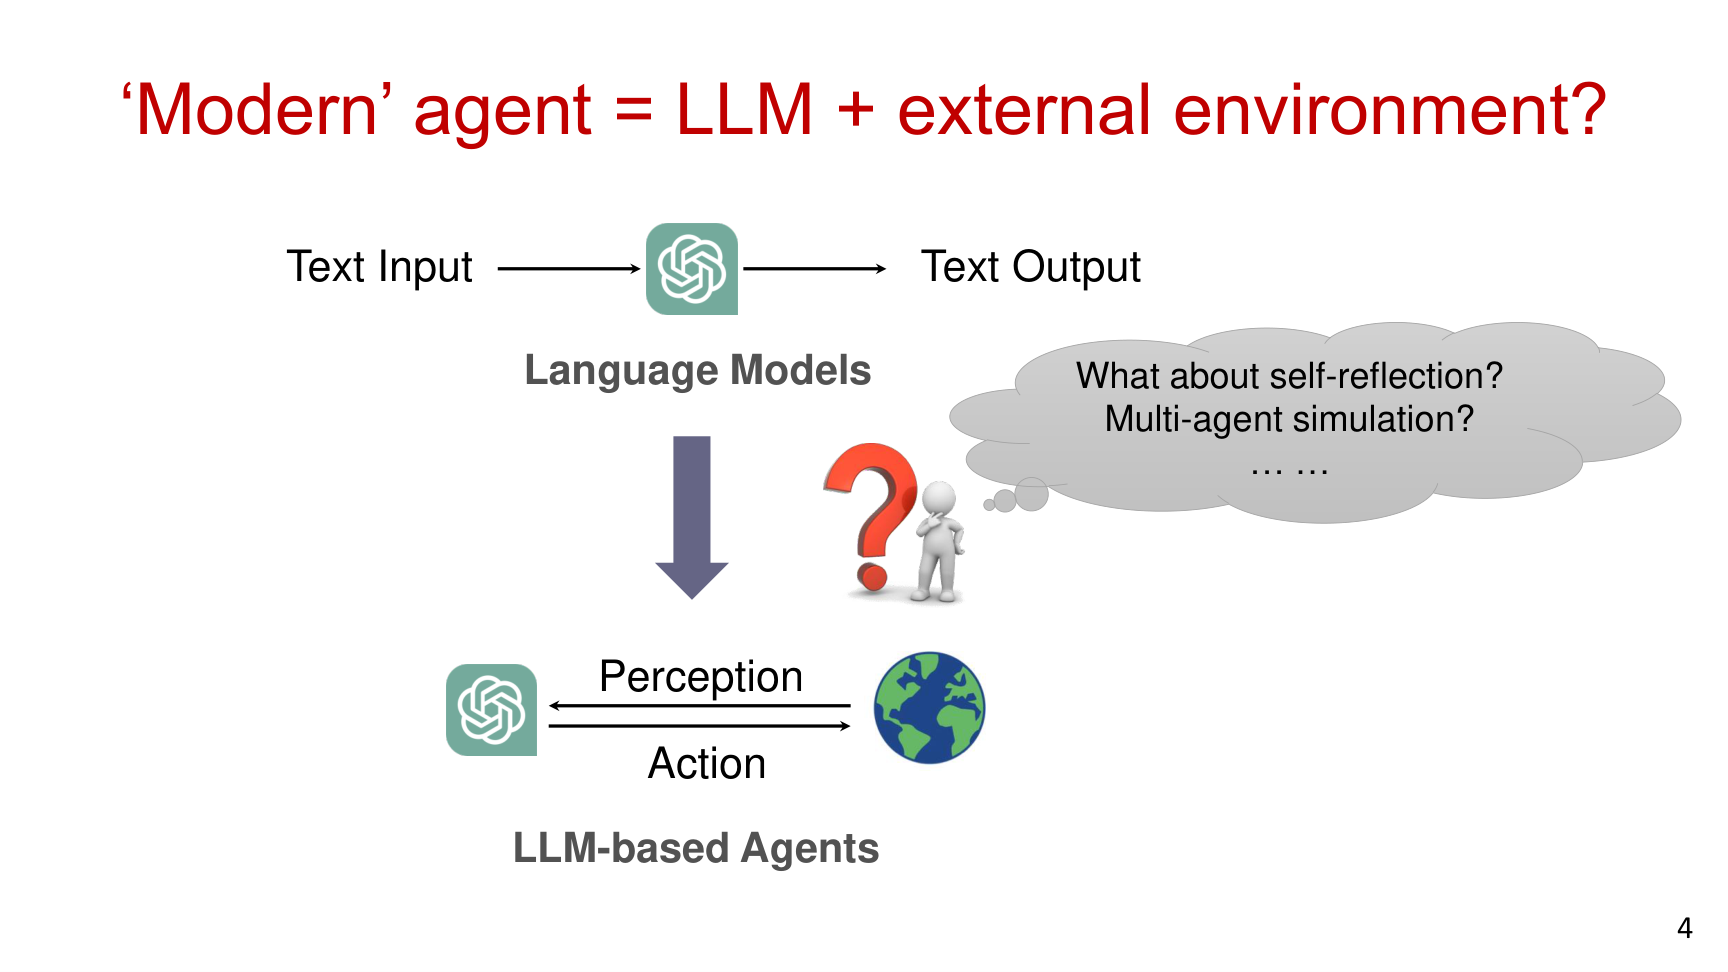
\includegraphics[width=0.82\textwidth]{../lectures/lec03_reasoning_memory_planning/figures/lec03_fig_001.png}
\caption{语言 agent 的最小闭环：perception、reasoning、action、self-reflection 和 environment feedback 共同构成 agent workflow。}
\end{figure}

这意味着“reasoning”本身也要重新定义。对语言 agent 来说，生成 token 不只是在输出答案，也可以是\textbf{内部动作（internal action）}：写计划、写状态假设、做自我反思、生成候选未来状态。这就是 Yu Su 强调 inner monologue 的原因。

\subsection{LLM-first 与 agent-first}

Lecture 中一个非常有用的区分是：
\begin{itemize}
\item \textbf{LLM-first view}：先有 LLM，再往上堆记忆、工具和 prompt scaffold，让它看起来像 agent。
\item \textbf{Agent-first view}：先从 agent 所需能力出发，再把 LLM 作为 reasoning / communication module 整合进去。
\end{itemize}

前者更贴近当下工程实践，后者更接近长期研究路线。Yu Su 没有简单否定任何一方，而是指出两者在系统设计中同时存在：今天的 agent 既是 prompt-heavy engineering artifact，也是朝着更完整智能体过渡的原型。

\subsection{为什么叫 language agent}

讲者用 logical agent、neural agent 和 language agent 的对比图强调：language agent 的突出特征不是它“更智能”，而是它拥有更高的\textbf{表达能力（expressiveness）}。逻辑 agent 很严谨但语言受限，纯神经 agent 可以编码很多模式但难以显式沟通，而 language agent 能用自然语言组织状态、理由、计划和工具调用。

\begin{figure}[H]
\centering
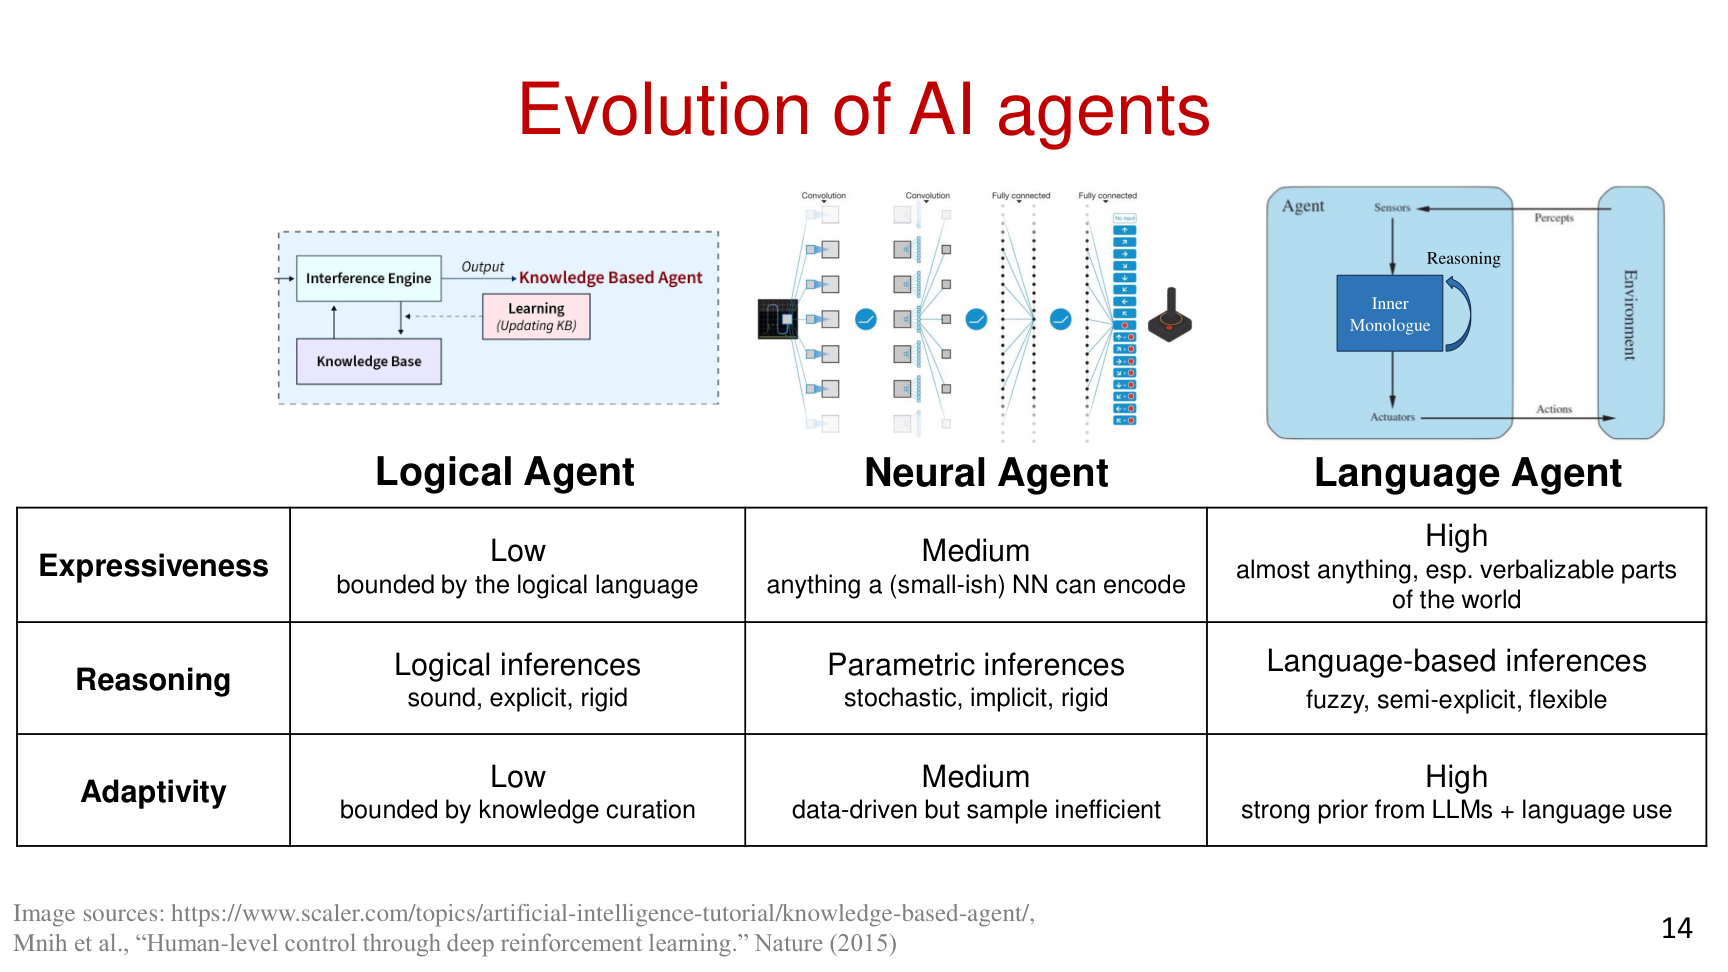
\includegraphics[width=0.78\textwidth]{../lectures/lec03_reasoning_memory_planning/figures/lec03_fig_002.png}
\caption{Logical / Neural / Language Agent 的对比：language agent 的核心优势是高表达性，这也解释了它为什么适合 reasoning、memory 和 planning 的协调。}
\end{figure}

\begin{knowledgebox}{本讲的统一视角}
语言不是附属接口，而是 language agent 的核心组织媒介。它既承载内隐或显式推理，也承载记忆索引、规划、协调、工具调用和人机沟通。
\end{knowledgebox}

\section{长期记忆：为什么当前 RAG 还不够}

\subsection{RAG 的问题不是“检索不够快”，而是“记忆结构太浅”}

Yu Su 用一个多跳问答案例说明当前 RAG 的典型失败：问题需要在多条知识之间做联想和桥接，但普通 dense retrieval 只会优先找到表面相似的片段，而不擅长 reconstruct deeper associations。

\begin{figure}[H]
\centering
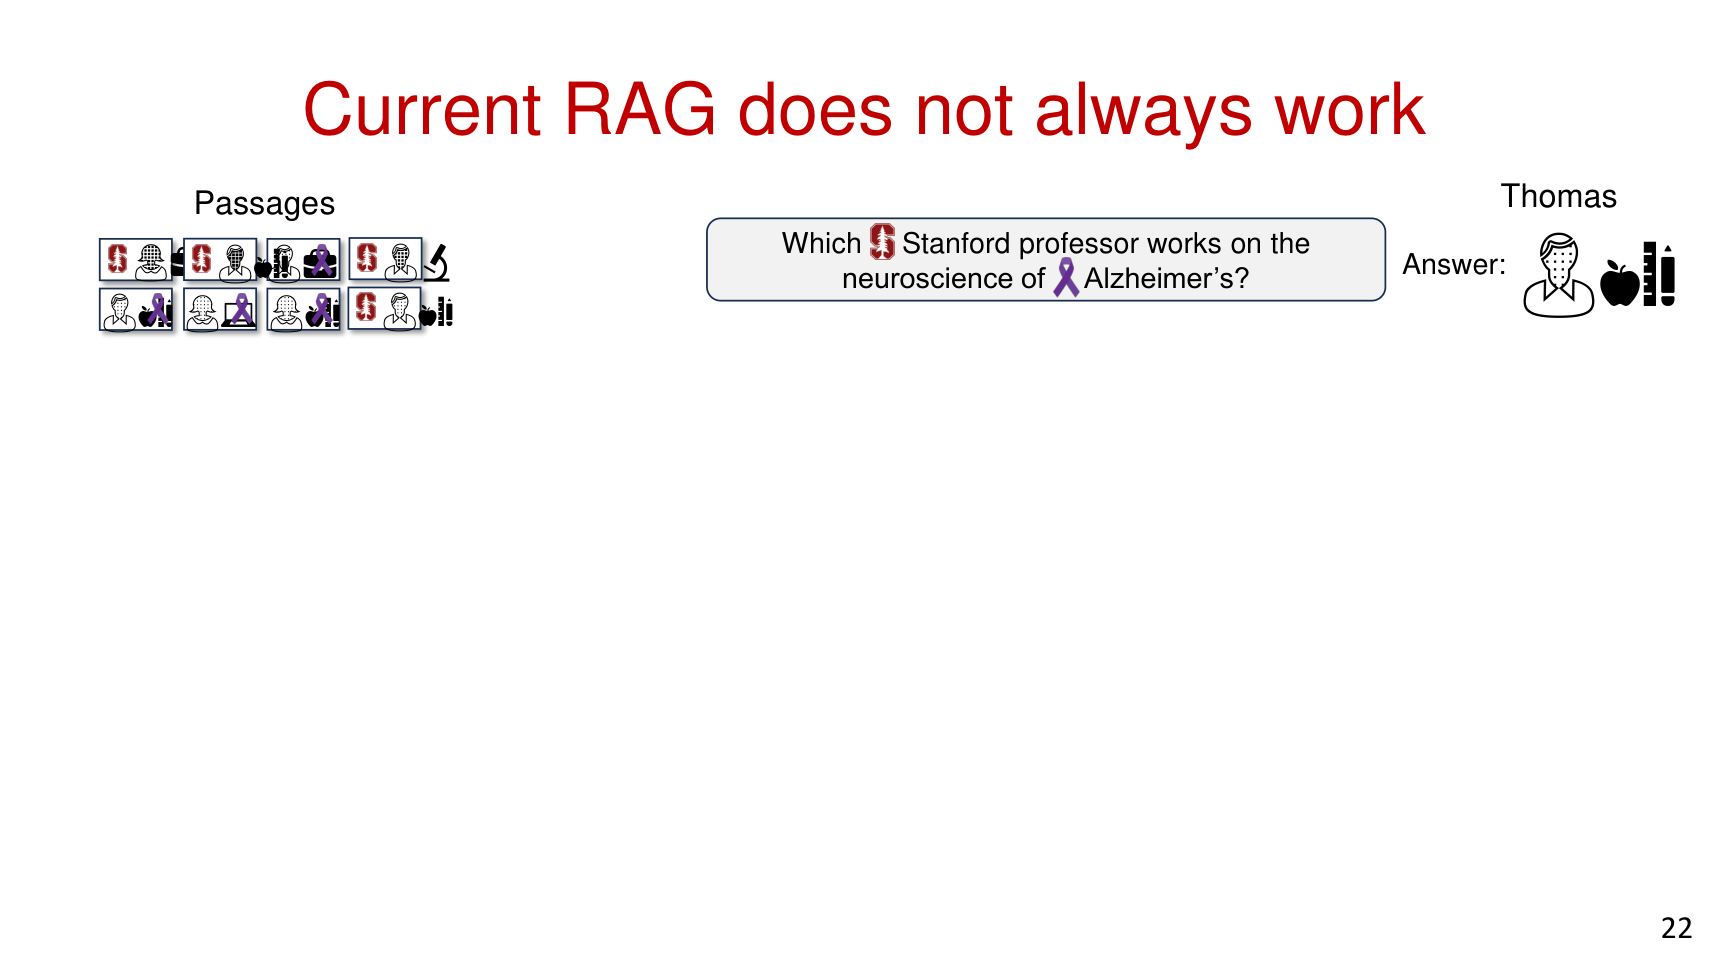
\includegraphics[width=0.78\textwidth]{../lectures/lec03_reasoning_memory_planning/figures/lec03_fig_003.png}
\caption{当前 RAG 的失败案例：多跳记忆问题被错误地退化成浅层相似性检索。}
\end{figure}

这意味着 language agent 的 memory 设计不能只停留在“外挂一些文档块然后 top-k 检索”。真正困难的是：\textbf{如何把新经验组织成可以联想、可恢复、可重组的 memory substrate。}

\subsection{HippoRAG：把长期记忆做成索引与联想系统}

HippoRAG 的核心灵感来自 hippocampal indexing theory。这个理论认为，海马体并不把完整记忆原样储存成单个块，而是维护索引以及记忆之间的联想关系，从而支持 pattern separation 和 pattern completion。

\begin{figure}[H]
\centering
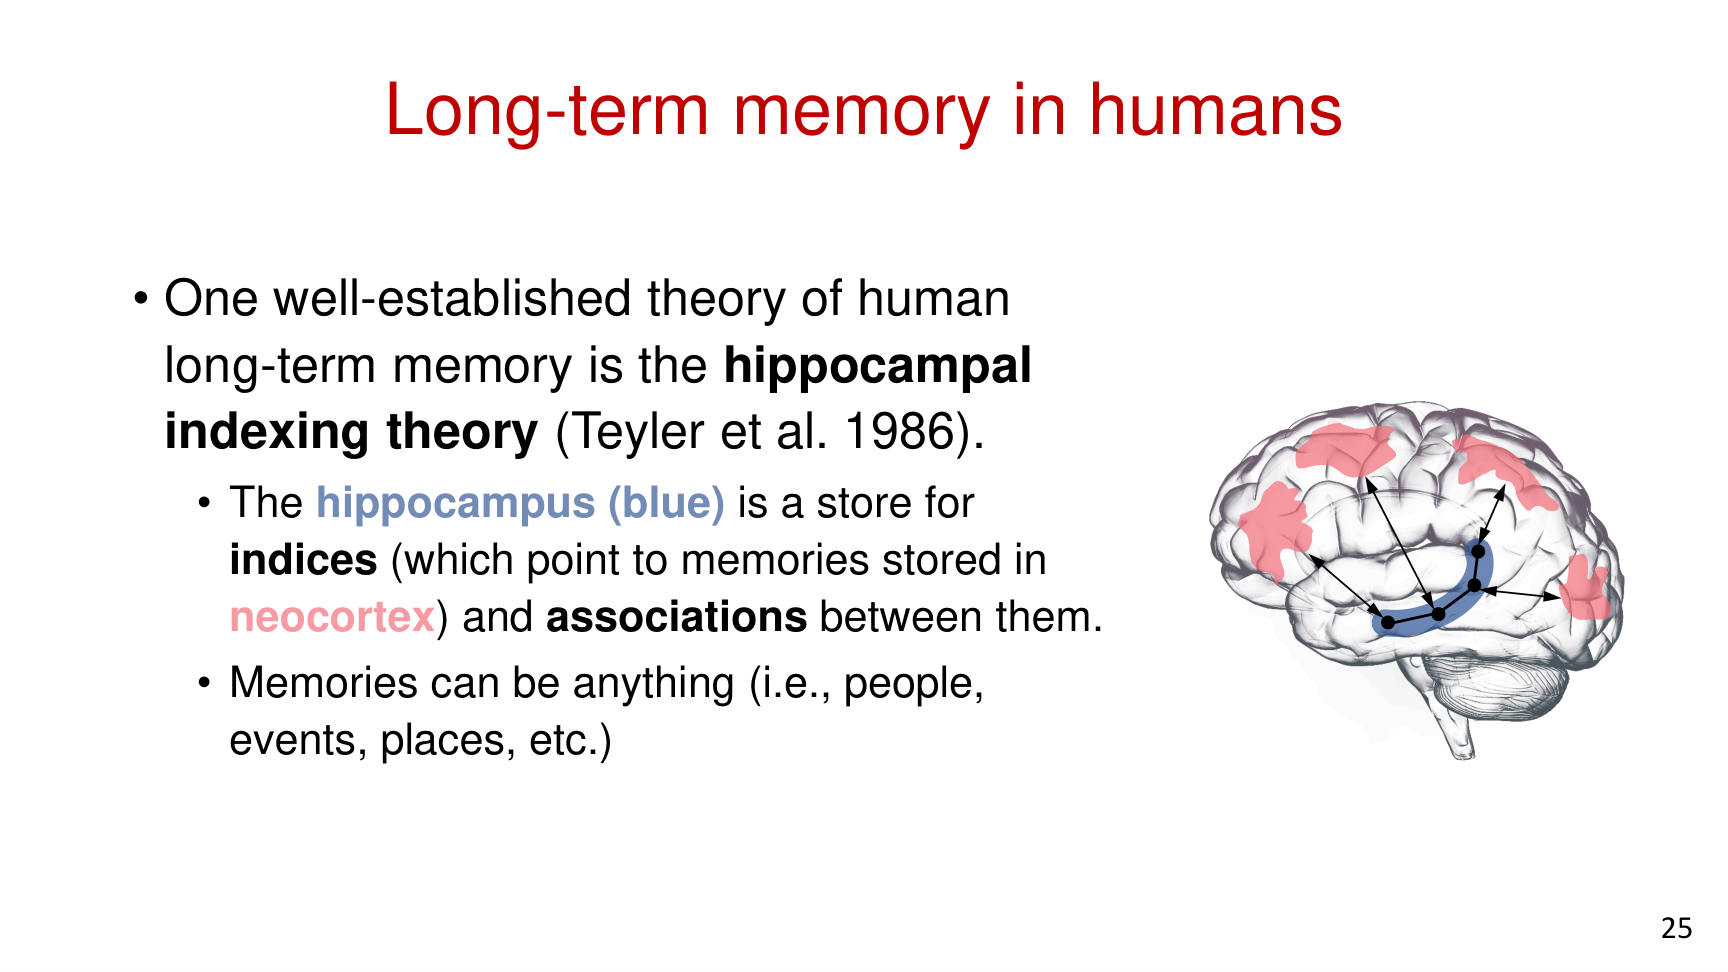
\includegraphics[width=0.74\textwidth]{../lectures/lec03_reasoning_memory_planning/figures/lec03_fig_004.png}
\caption{HippoRAG 的认知灵感：长期记忆不是只靠相似度召回，而是靠索引和联想结构恢复。}
\end{figure}

这给语言 agent 一个关键启示：如果记忆是图结构而不是平铺 chunk 列表，那么 retrieval 就不仅是“哪个段落最像 query”，而是“从哪些锚点出发，沿哪些关系扩散，才能恢复与当前任务相关的完整记忆”。

HippoRAG 用知识图、LLM 和 Personalized PageRank 来实现这一点。一个简化写法是：
\[
\mathbf{r}=\alpha \mathbf{e}_q + (1-\alpha)\mathbf{P}^{\top}\mathbf{r}
\]
这里 $\mathbf{e}_q$ 是由查询初始化的 personalization 向量，$\mathbf{P}$ 是知识图转移矩阵，$\mathbf{r}$ 是最终 memory relevance 分布，$\alpha$ 控制查询锚点与图扩散之间的权衡。

\paragraph{直觉解释}
普通 RAG 更像“把问题拿去最近邻检索”；HippoRAG 更像“先找到与问题相关的记忆入口，再沿着联想路径逐渐恢复整片相关记忆结构”。

\begin{figure}[H]
\centering
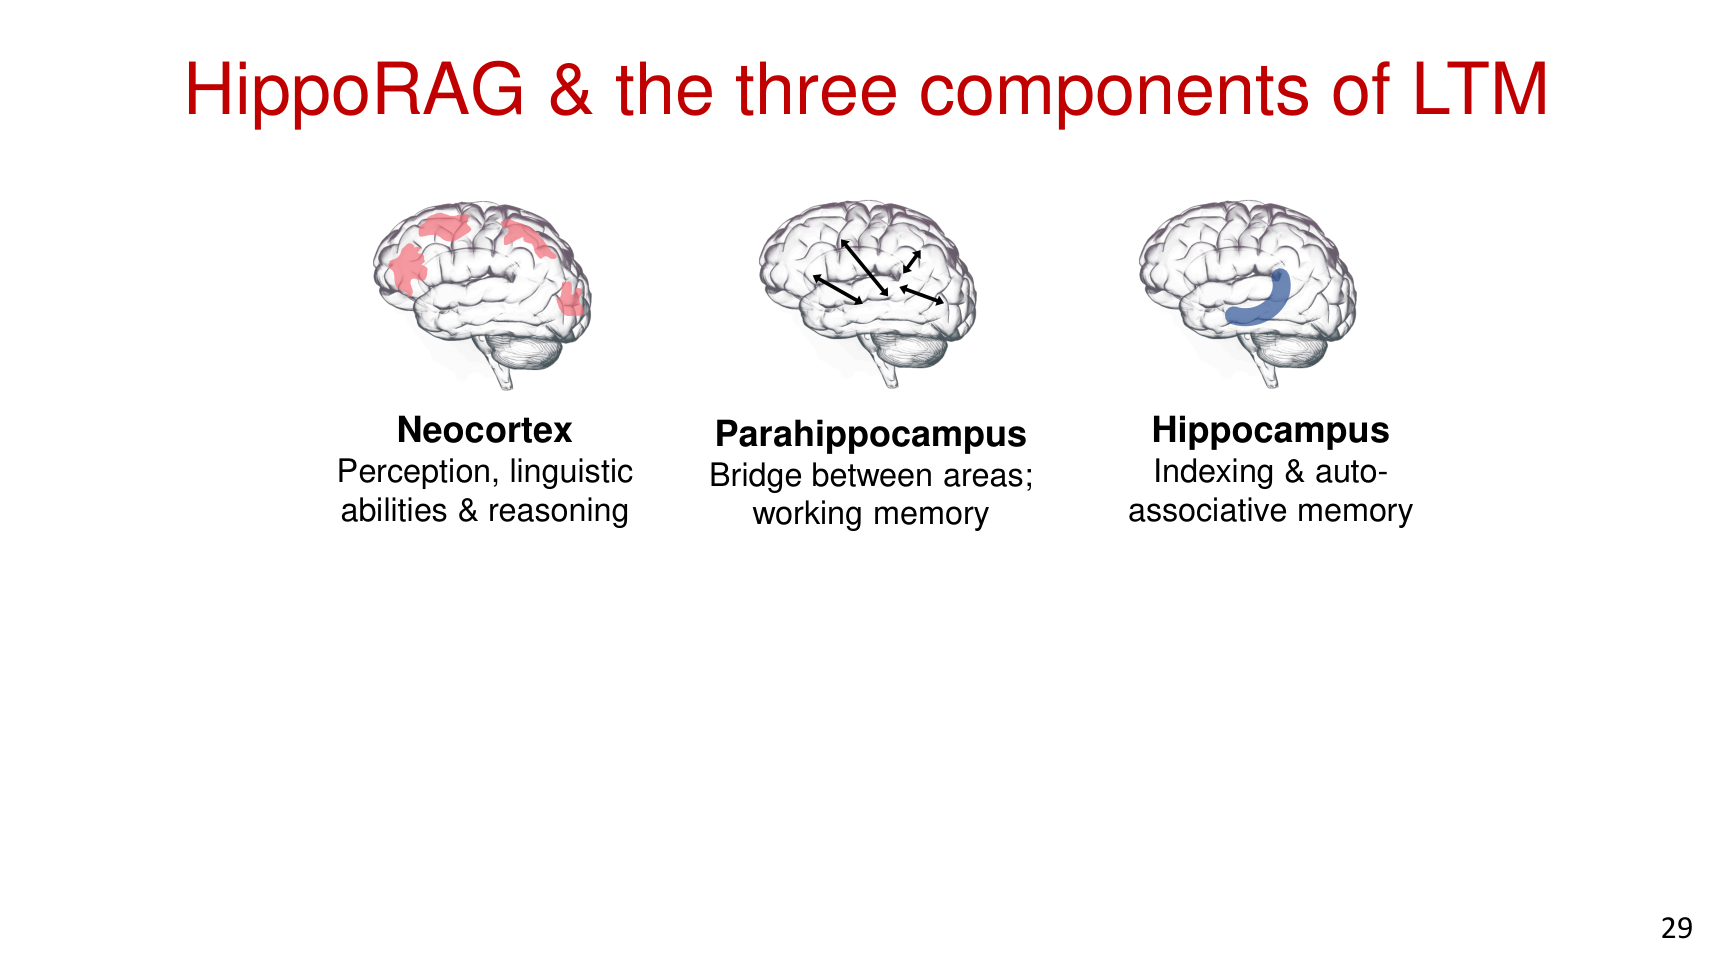
\includegraphics[width=0.80\textwidth]{../lectures/lec03_reasoning_memory_planning/figures/lec03_fig_005.png}
\caption{HippoRAG 的三个部件：知识存储、桥接与索引-联想机制共同组成长期记忆检索系统。}
\end{figure}

\begin{lstlisting}
Build a graph over entities, passages, and relations
Seed query-relevant nodes from the current question
Run Personalized PageRank over the graph
Retrieve passages associated with the highest-scoring memory nodes
\end{lstlisting}

\paragraph{为什么这对 agent 很关键}
对 language agent 来说，记忆不是只服务单轮问答。它还要支撑个性化、持续学习、多步任务和跨时空的关联恢复。没有更好的记忆结构，agent 很容易每轮都像第一次见到世界。

\subsection{HippoRAG 的实验结果与边界}

HippoRAG 在多跳问答上明显优于常见 RAG baselines，也往往比迭代检索更便宜。这说明非参数记忆并不是无用，而是要设计得像\textbf{联想记忆系统}，而非简单文本外挂。

\begin{figure}[H]
\centering
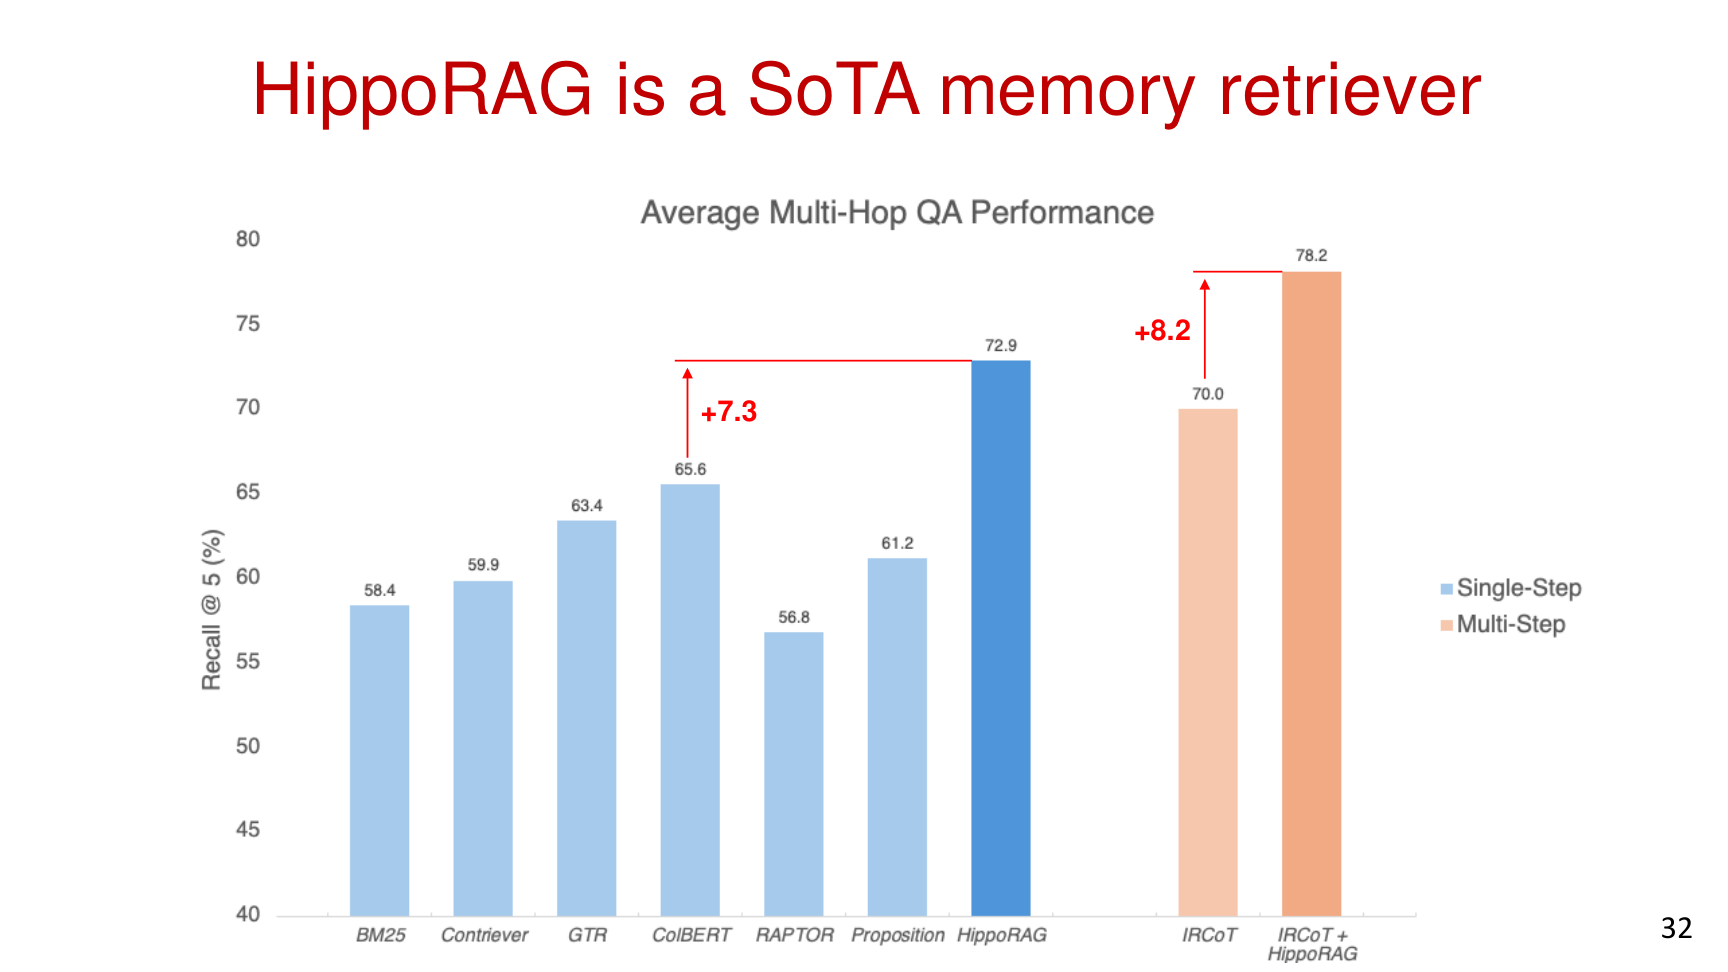
\includegraphics[width=0.72\textwidth]{../lectures/lec03_reasoning_memory_planning/figures/lec03_fig_006.png}
\caption{HippoRAG 的结果页：记忆检索结构本身就会显著影响 reasoning quality。}
\end{figure}

但讲者也没有把它说成完整答案。HippoRAG 仍然主要解决“如何更好地取回长期记忆”，并不自动解决 continual learning、memory editing、personalization safety 等更广问题。它是 memory module 的强基线，而不是终局。

\section{推理：显式 CoT 之外，implicit reasoning 依然重要}

\subsection{为什么要讨论 implicit reasoning}

当整个社区都在关注 CoT 时，Yu Su 反过来问：没有 verbalized thoughts 的 transformer，是否也能通过参数内部结构学会推理？这就是 Grokked Transformers 的研究对象。

\begin{figure}[H]
\centering
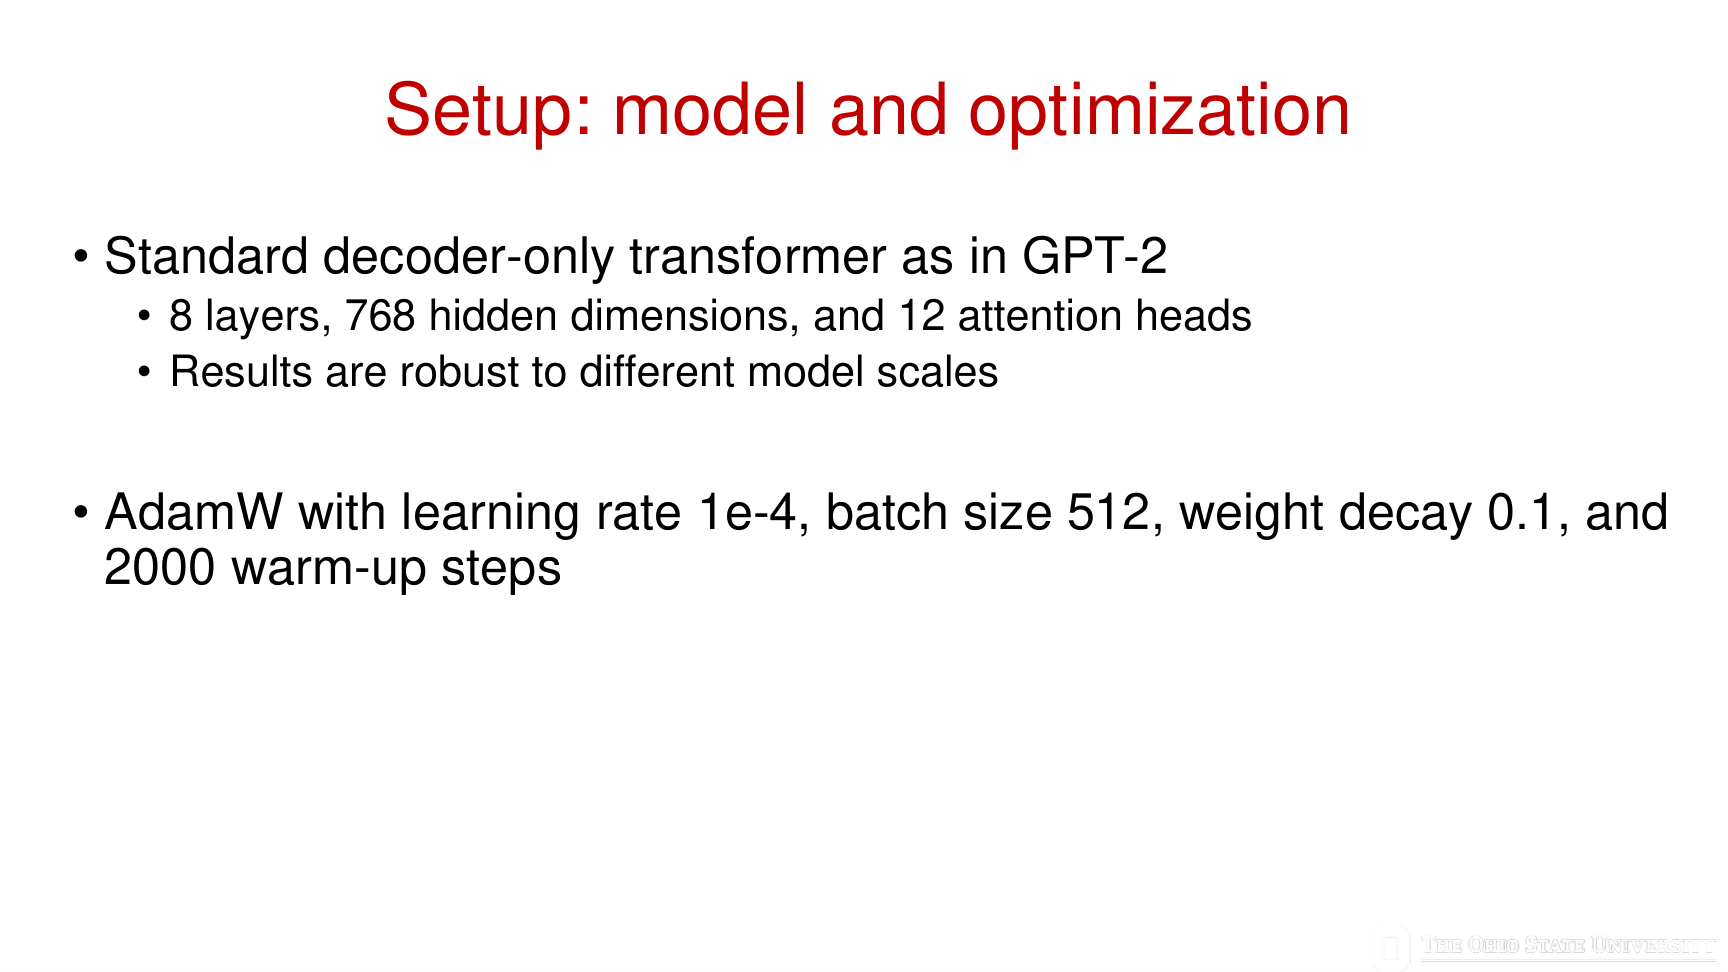
\includegraphics[width=0.80\textwidth]{../lectures/lec03_reasoning_memory_planning/figures/lec03_fig_007.png}
\caption{Grokked Transformers 的实验设置：通过可控合成任务，单独研究 implicit reasoning 的学习与泛化。}
\end{figure}

这里的重点是，language agents 的 reasoning 不应该被误解为“只要会写 CoT”。在很多时候，显式 CoT 是\textbf{外显接口}，而真正的结构化表征学习仍然发生在模型参数与电路层面。若忽略这一点，就会把推理能力过度等同于解释能力。

\subsection{Grokking：从记忆回放到泛化相变}

Grokked Transformers 研究显示，transformer 可以学会 implicit reasoning，但往往要经历 grokking：也就是在训练误差早已很低之后，继续训练很久，模型才从 memorization 过渡到真正 generalization。

\begin{figure}[H]
\centering
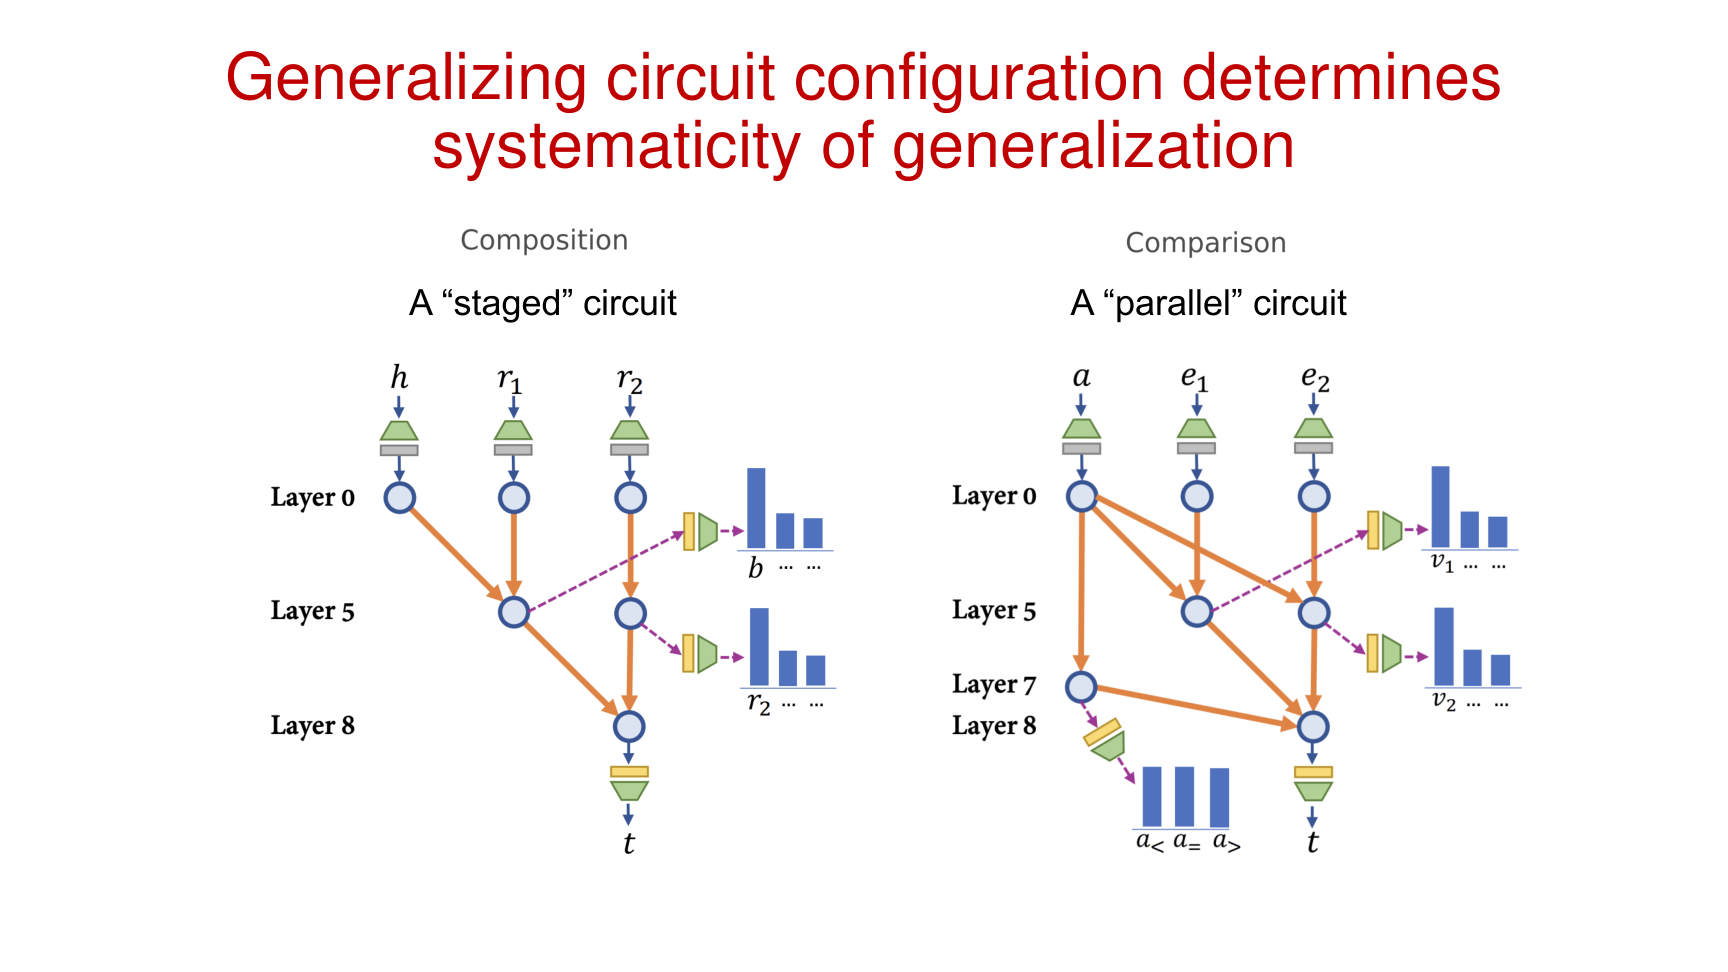
\includegraphics[width=0.78\textwidth]{../lectures/lec03_reasoning_memory_planning/figures/lec03_fig_008.png}
\caption{generalizing circuit 的配置决定 systematicity：不同 reasoning type 会形成不同的内部电路结构。}
\end{figure}

\begin{figure}[H]
\centering
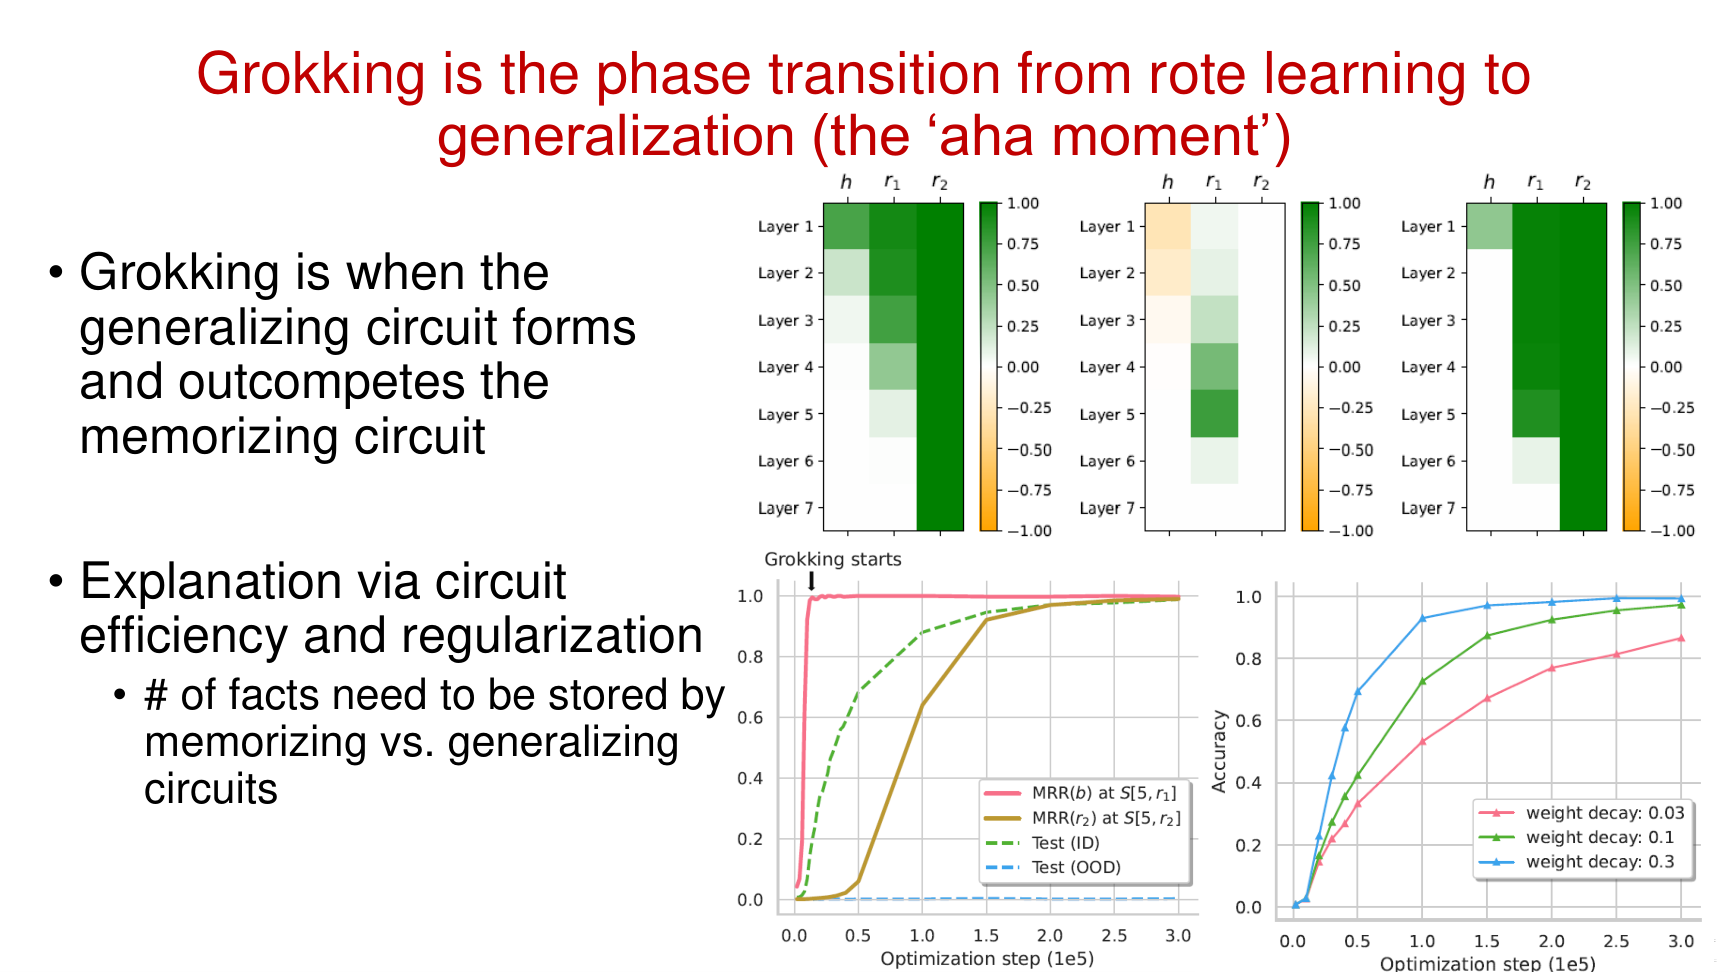
\includegraphics[width=0.78\textwidth]{../lectures/lec03_reasoning_memory_planning/figures/lec03_fig_009.png}
\caption{Grokking 被讲成从 rote memorization 向 systematic generalization 的相变。}
\end{figure}

\begin{lstlisting}
Train the transformer far beyond interpolation
Probe intermediate representations with a logit lens
Run causal tracing to identify memorizing and generalizing circuits
Compare circuit configurations across reasoning types
\end{lstlisting}

\paragraph{为什么这件事与 language agents 有关}
因为很多 agent 成功与否，取决于模型是否已经学会某种\textbf{隐式结构能力}。如果底层模型连 relations、rules、state abstractions 都没学稳，那么上层再复杂的 planning scaffold 也只是补丁。

\paragraph{一个重要 caveat}
Yu Su 也强调，Grokked Transformers 的证据来自可控 synthetic settings。它告诉我们“这种能力机制存在”，但不意味着大模型在开放世界里已经自动拥有同等稳健的 implicit reasoning。

\section{规划：从 reactive execution 到 model-based planning}

\subsection{Planning setting 已经变了}

传统规划常假定 formal domain、有限动作空间和清晰 goal test。但 language agents 进入 web、travel、GUI 等环境后，goal 用自然语言表达，动作空间开放且状态常带噪声。于是 planning 不再是单纯求解 PDDL，而是要处理含糊目标、开放动作、多模态反馈和昂贵环境交互。

\begin{figure}[H]
\centering
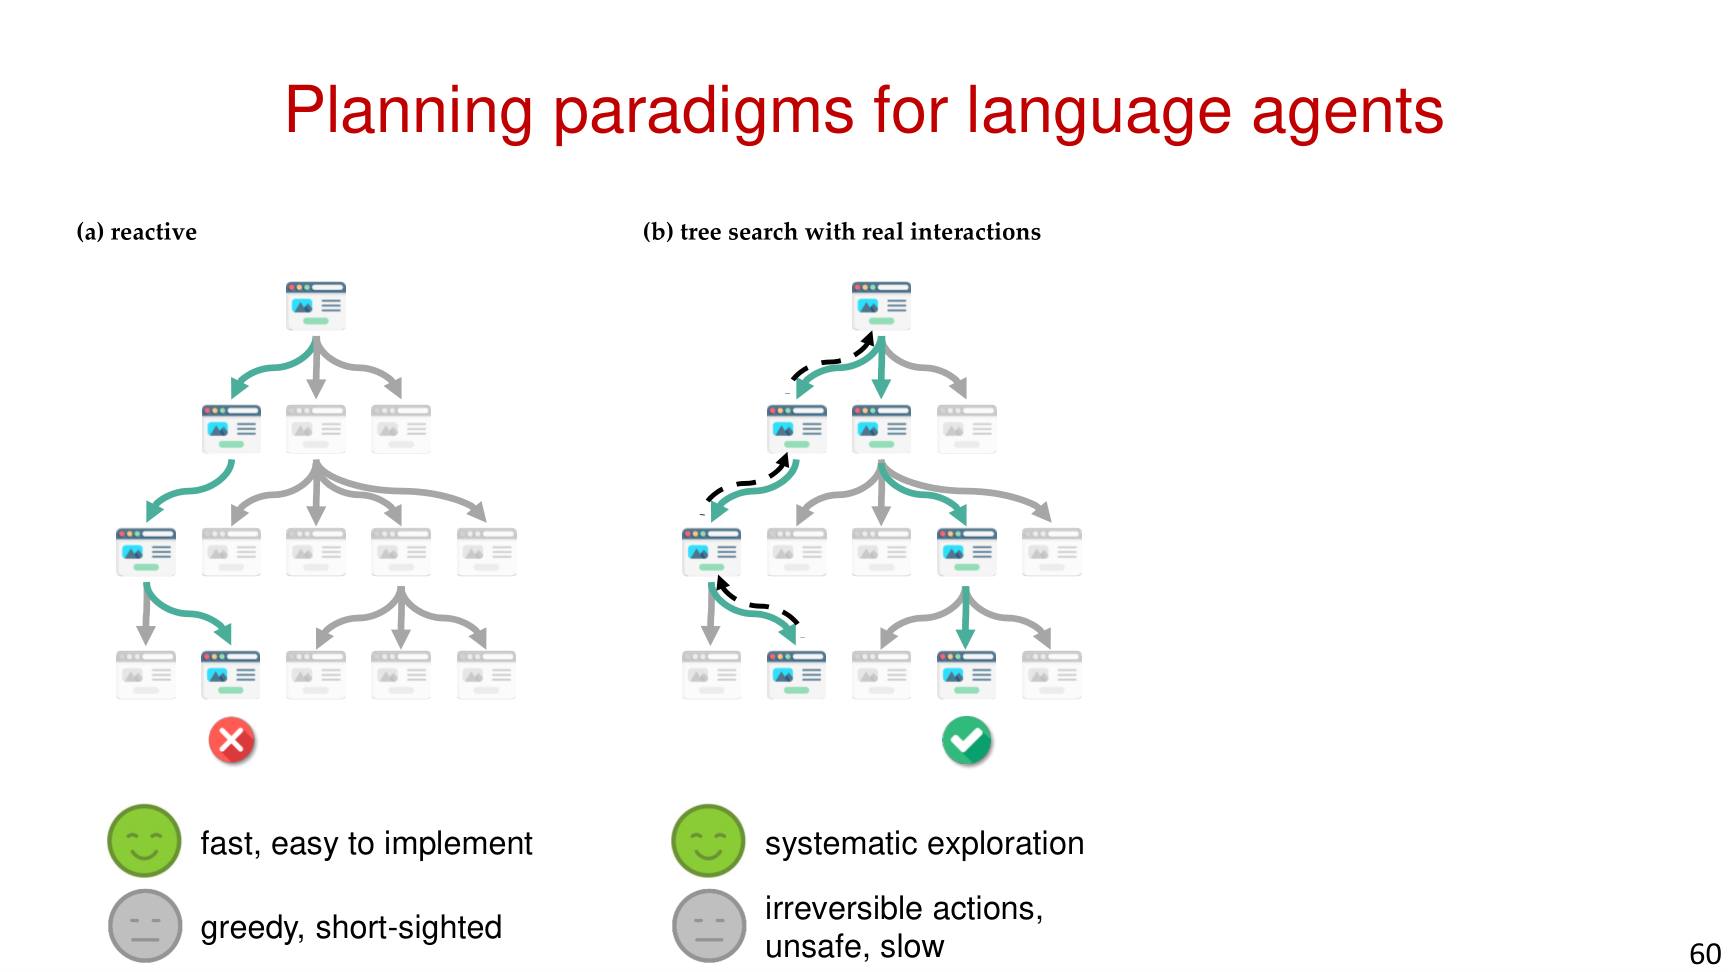
\includegraphics[width=0.78\textwidth]{../lectures/lec03_reasoning_memory_planning/figures/lec03_fig_010.png}
\caption{Planning paradigms 对比：reactive planning 快但短视，tree search 更系统但在真实环境中常太慢、太危险。}
\end{figure}

Yu Su 用 reactive、tree search 与 model-based planning 的比较说明：在真实网页环境里，单纯 tree search 面临三重问题：
\begin{itemize}
\item 很多动作是\textbf{不可逆}的，无法随意 backtrack。
\item 真环境交互带来\textbf{安全和隐私风险}。
\item 在线探索会显著增加 latency 与 cost。
\end{itemize}

\begin{figure}[H]
\centering
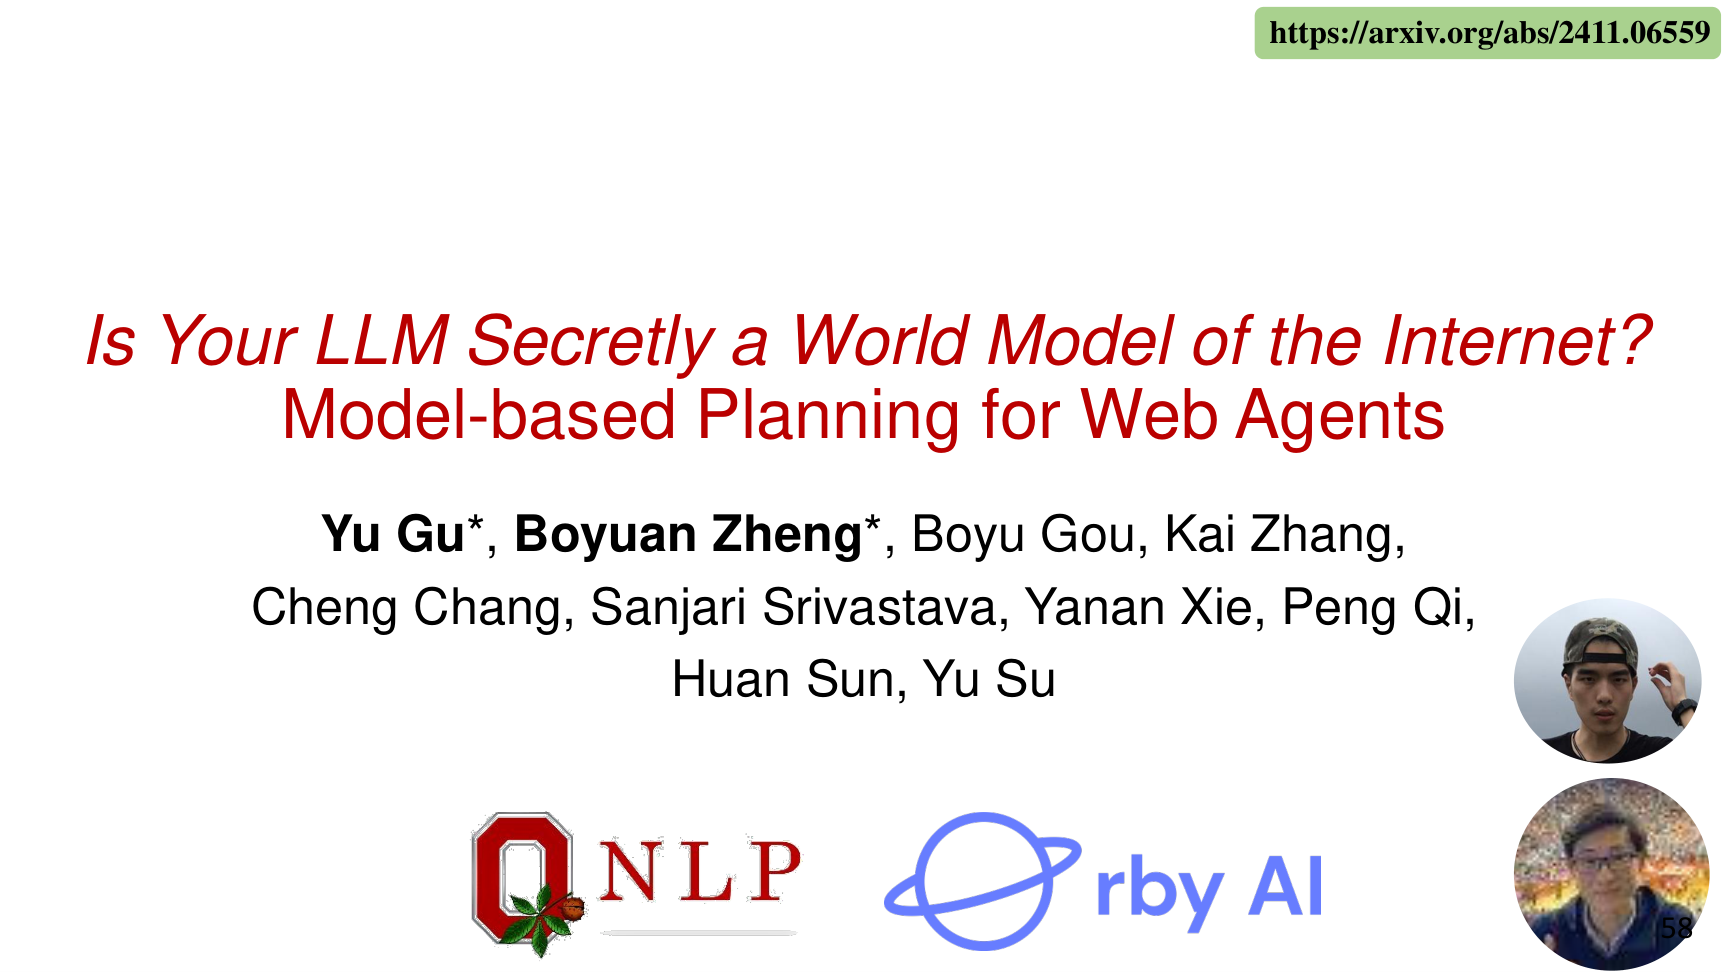
\includegraphics[width=0.76\textwidth]{../lectures/lec03_reasoning_memory_planning/figures/lec03_fig_011.png}
\caption{WebDreamer 连接 benchmark 视角与 planning 视角：web agent 不只是能点网页，而是要在现实约束下做安全高效规划。}
\end{figure}

\subsection{WebDreamer：先在脑内做 imagination，再去网页上行动}

WebDreamer 的关键思想是：既然真实环境探索昂贵且危险，那就训练一个\textbf{world model} 先预测动作后果，再根据预测结果选择动作。

\[
\hat{T}: \mathcal{S}\times \mathcal{A}\rightarrow \mathcal{S}
\]
这里 $\mathcal{S}$ 是状态空间，$\mathcal{A}$ 是动作空间，$\hat{T}$ 是世界模型。它回答的问题非常具体：如果在当前状态 $s_t$ 下执行动作 $a_t$，下一个状态会是什么？

进一步，planner 可以写成：
\[
a_t^{\star}=\arg\max_{a_t\in \mathcal{A}(s_t)} \hat{V}\!\left(\hat{T}(s_t,a_t)\right)
\]
其中 $\hat{V}$ 是对预测后继状态的价值评估器。

\begin{figure}[H]
\centering
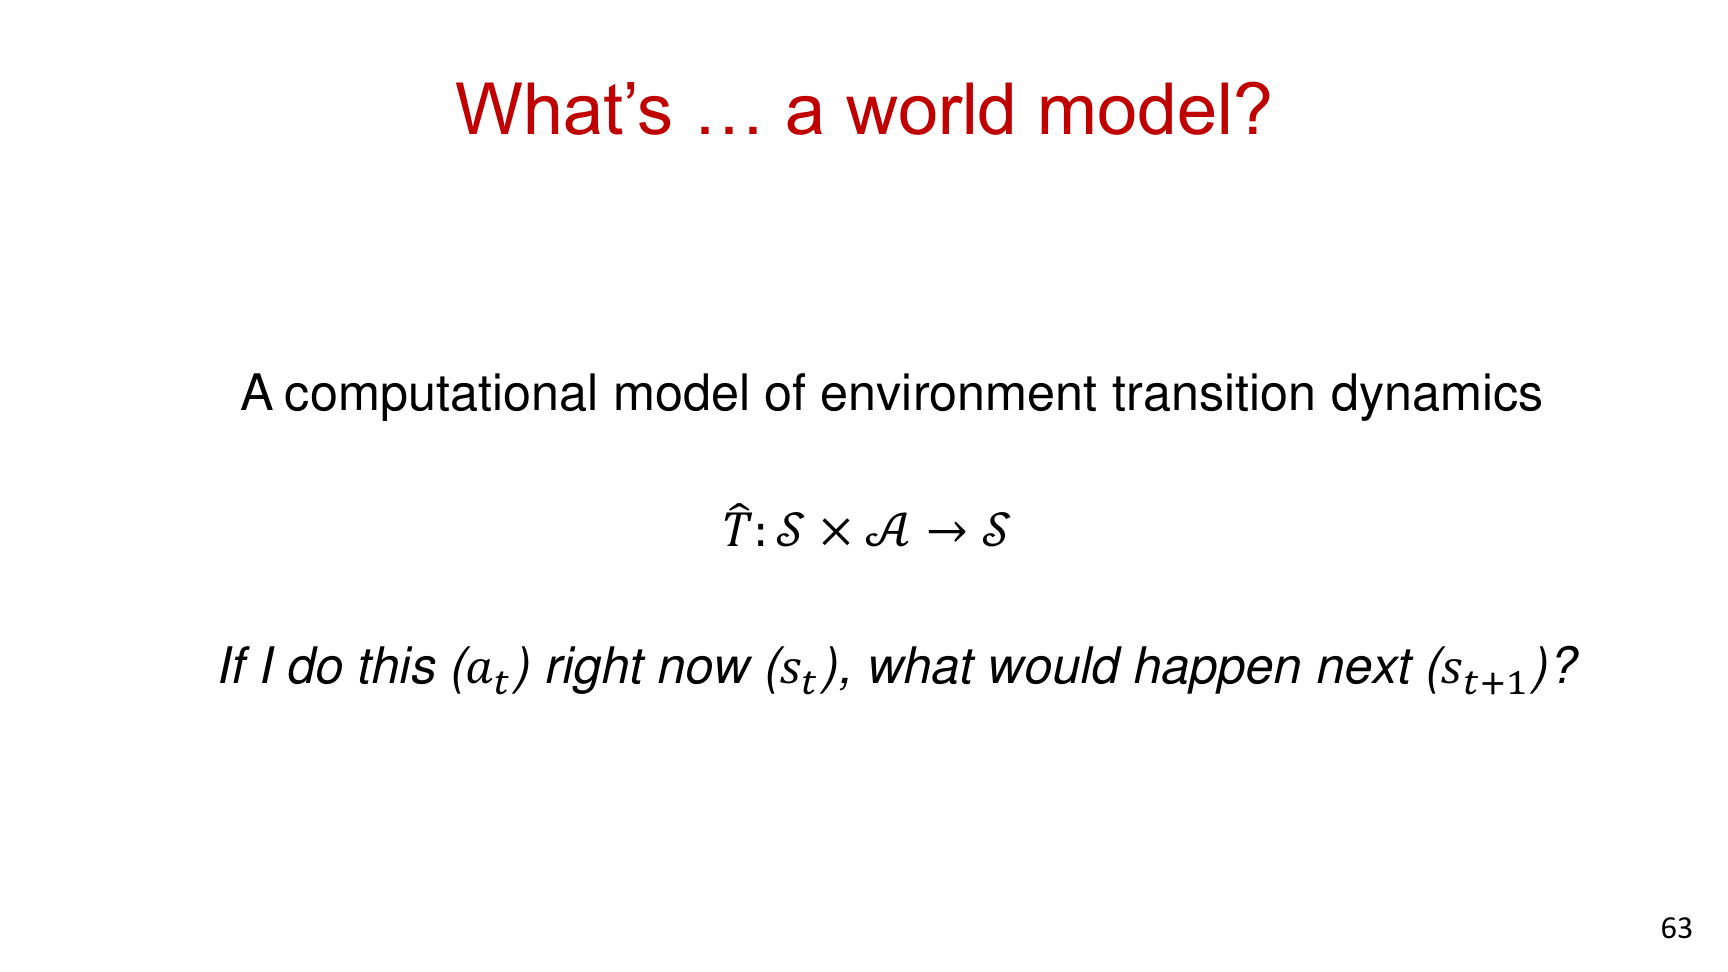
\includegraphics[width=0.74\textwidth]{../lectures/lec03_reasoning_memory_planning/figures/lec03_fig_012.png}
\caption{World model 的最小抽象：在执行动作前先预测状态转移。}
\end{figure}

\begin{figure}[H]
\centering
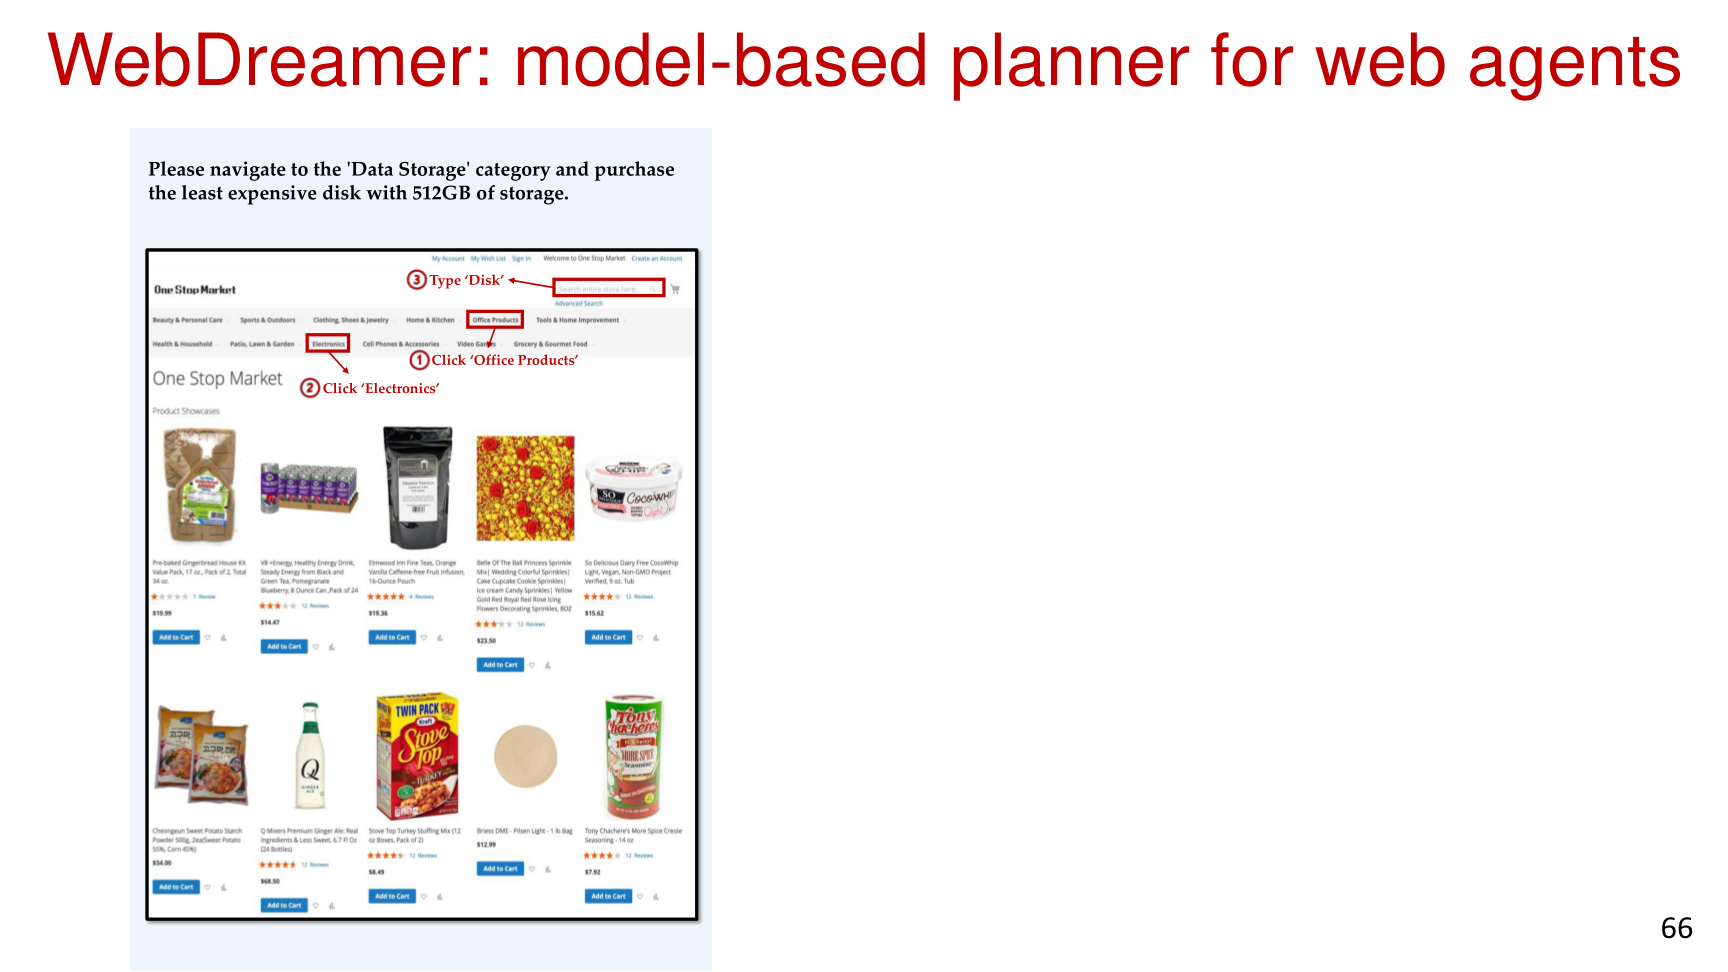
\includegraphics[width=0.78\textwidth]{../lectures/lec03_reasoning_memory_planning/figures/lec03_fig_013.png}
\caption{WebDreamer 的示例：agent 先在内部模拟网页跳转和后续选项，再决定是否真的点击。}
\end{figure}

\begin{lstlisting}
Observe the current webpage state s_t
Enumerate candidate actions
Predict successor states with the world model
Score predicted states with a value function
Execute the best action in the real environment
\end{lstlisting}

\paragraph{为什么这比 reactive planning 更像“高级 agent”}
因为 agent 不再只凭当前页面做局部反应，而是把语言模型用作 environment simulator。它先在内部世界里想象未来，再决定是否把动作提交给外部世界。这与人类 planning 的基本直觉非常接近。

\paragraph{为什么这比 tree search 更现实}
Tree search 假设你可以大量试错；WebDreamer 假设现实里试错有代价，因此应该把更多搜索移入 learned world model。这正是 language agent planning 与纯 benchmark search 的关键区别。

\section{整合视角：memory、reasoning、planning 为什么必须一起看}

\begin{figure}[H]
\centering
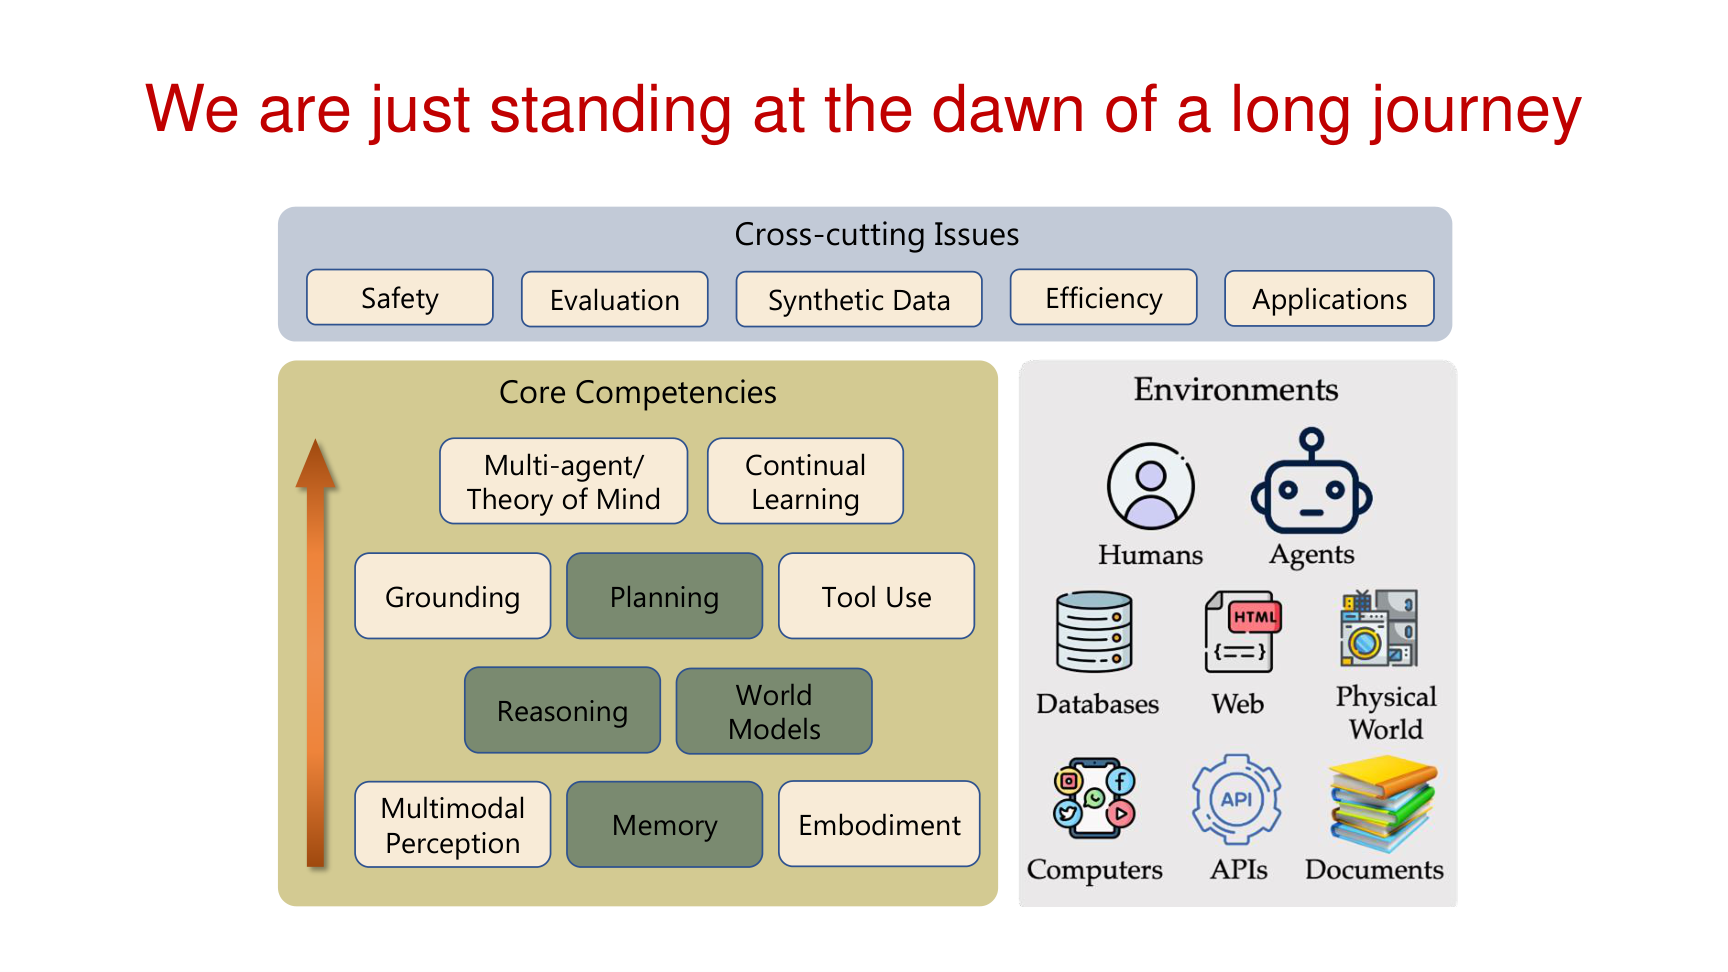
\includegraphics[width=0.82\textwidth]{../lectures/lec03_reasoning_memory_planning/figures/lec03_fig_014.png}
\caption{语言 agent 能力地图：memory、reasoning、world models、planning、grounding、tool use、continual learning 共同构成系统能力。}
\end{figure}

Yu Su 在结尾最重要的贡献，是把 memory、reasoning、planning 重新组织成一个统一能力版图：
\begin{itemize}
\item \textbf{Memory} 决定 agent 能否跨时空整合经验。
\item \textbf{Reasoning} 决定 agent 能否形成和操作抽象状态。
\item \textbf{Planning / World Models} 决定 agent 能否在执行前进行 simulation 与 deliberation。
\end{itemize}

这三者并不是相互独立的。没有 memory，planning 会失忆；没有 reasoning，memory 只剩检索；没有 world model，reasoning 无法稳健转化为行动策略。

\begin{figure}[H]
\centering
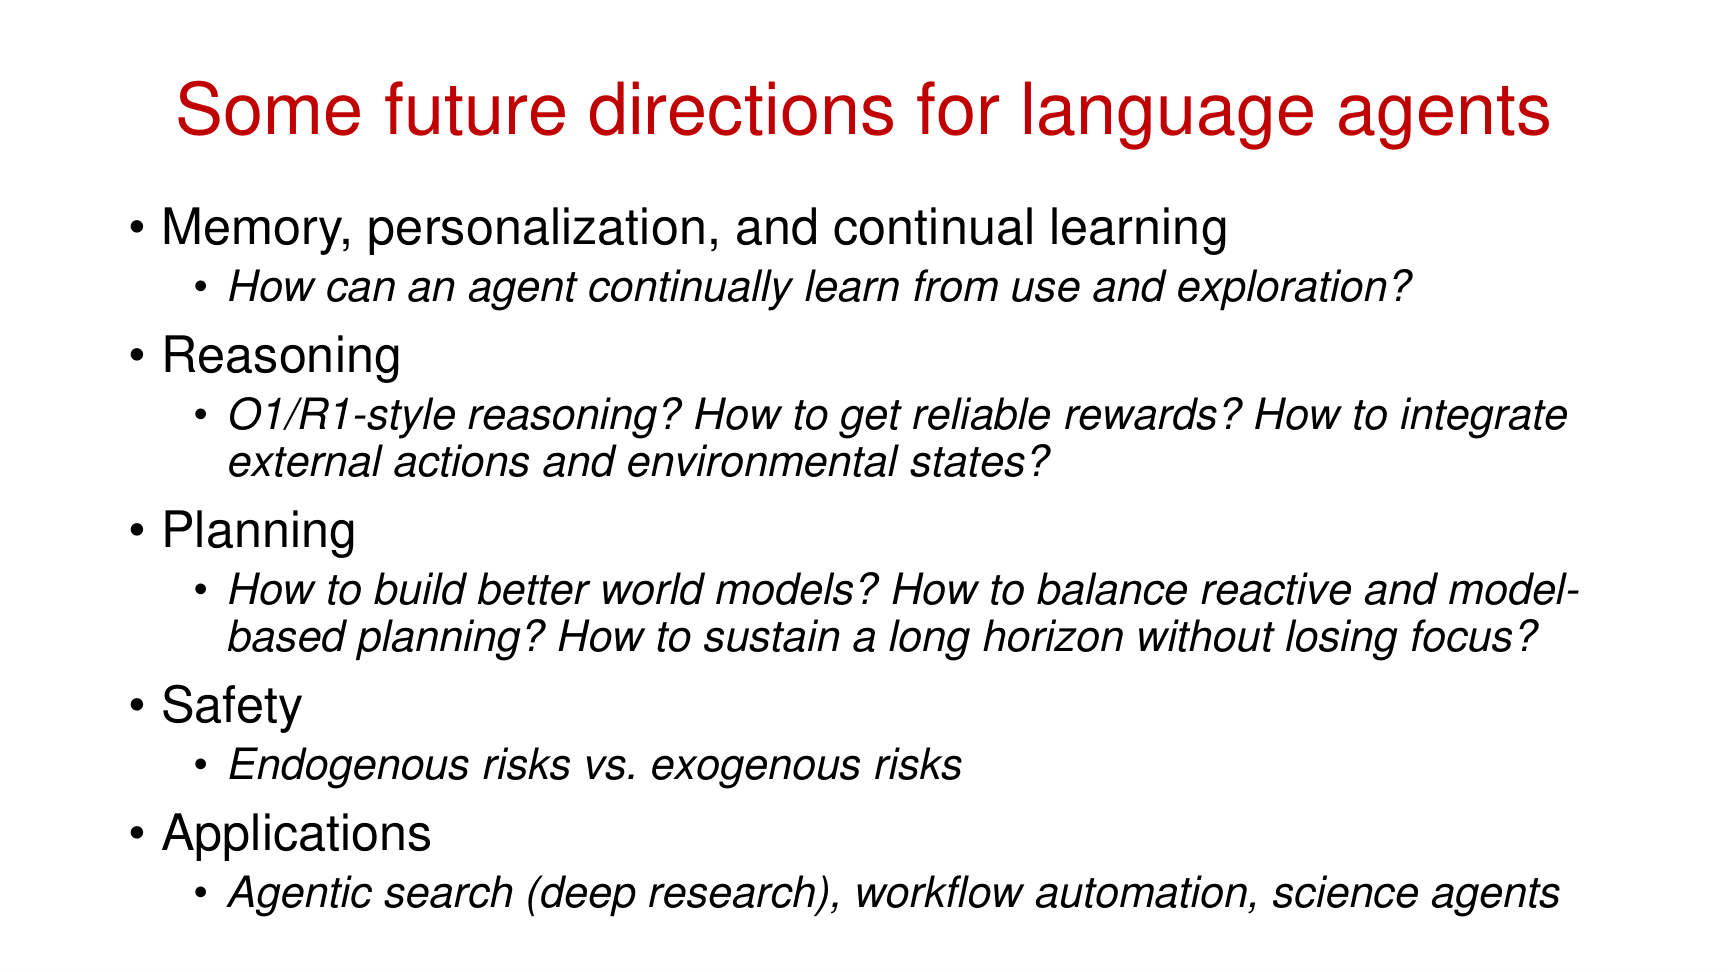
\includegraphics[width=0.80\textwidth]{../lectures/lec03_reasoning_memory_planning/figures/lec03_fig_015.png}
\caption{未来方向页：个性化记忆、持续学习、可靠 reasoning reward、grounding 和规划将共同定义下一代 language agents。}
\end{figure}

\section{与 readings 的连接}

\subsection{HippoRAG：记忆不是外挂，而是结构能力}

HippoRAG reading 让本讲的记忆部分有了非常清晰的技术落点。它说明长期记忆不是“有没有更多文档”，而是“agent 是否有足够好的记忆索引与联想机制”。对自学者来说，这个 reading 也是理解为什么 current RAG 不足以支撑真正 agent memory 的最好入口。

\subsection{Grokked Transformers：显式与隐式推理必须一起讨论}

Grokked Transformers reading 的价值，在于它把隐式推理从抽象命题变成了可分析的电路问题。它提醒我们：对 language agents 来说，显式 CoT 只是接口层；更深层的 reasoning 能力还取决于模型内部能否学到 generalizing circuits。

\subsection{WebDreamer：规划的成本结构发生了变化}

WebDreamer reading 则把 planning 讨论从“会不会 search”推进到“什么时候该在内部 world model 中 search，什么时候才去真实环境执行”。这对 web / GUI / OS agents 尤其关键，因为环境交互有成本且可能不可逆。

\section{失败模式与前后讲联系}

\subsection{本讲最重要的失败模式}

\begin{enumerate}
\item \textbf{把 agent 只当成 workflow wrapper。} 这样会看不到 memory、reasoning、planning 的结构问题。
\item \textbf{把 RAG 当成长期记忆的完整答案。} 浅层检索无法替代联想与索引机制。
\item \textbf{把 CoT 当成全部推理。} 没有 implicit reasoning substrate，再多 verbal thoughts 也可能只是表演。
\item \textbf{在真实环境中过度依赖在线 tree search。} 成本、不可逆性和安全风险会迅速失控。
\item \textbf{把 world model 想象成完美模拟器。} 如果预测误差太大，model-based planning 反而会系统性误导行动。
\end{enumerate}

\subsection{与前后讲的联系}

前两讲主要讨论 reasoning 本身：第一讲关注 inference-time search，第二讲关注 training-time judge。Yu Su 这讲把视角放大到完整 language agent：reasoning 不再只是生成思维链，而是与 memory organization 和 world-model planning 一起构成 agent intelligence。后续 multimodal、theorem proving、安全与抽象发现等讲次，其实都能放进这个框架里继续展开。

\section{本章小结}

如果把本讲压缩成一句话，就是：
\begin{center}
\emph{language agent 的核心不是“会说话”，而是能用语言组织记忆、进行推理、模拟未来并协调行动。}
\end{center}

Yu Su 通过 HippoRAG、Grokked Transformers 和 WebDreamer 给出三条清晰主线：
\begin{itemize}
\item 记忆要从浅层检索升级成结构化联想系统。
\item 推理既有显式外显层，也有隐式参数电路层。
\item 规划要从 reactive execution 走向 model-based deliberation。
\end{itemize}

对整门课而言，这一讲相当于给“advanced LLM agents”补上了系统架构视角：单点优化某个 prompt 或某个 benchmark 技巧远远不够，真正的难点在于如何让 memory、reasoning、planning 在同一 agent 中形成闭环。

\section{复习题}

\begin{enumerate}
\item 为什么 Yu Su 坚持使用 “language agent” 而不是泛泛的 AI agent？
\item 当前 RAG 在多跳记忆问题上的主要缺陷是什么？
\item HippoRAG 为什么要用图结构和 Personalized PageRank，而不是只做 dense retrieval？
\item Grokking 为什么说明 implicit reasoning 与 generalization 有深层联系？
\item WebDreamer 与 reactive web agent 的最关键区别是什么？
\end{enumerate}

\section{深入思考题}

\begin{enumerate}
\item 如果 world model 预测常常不准，agent 应该如何在真实环境反馈与内部模拟之间做校准？
\item 对长期个性化 agent 来说，memory retrieval、memory editing 与 privacy control 应该如何共同设计？
\item 你是否认同“显式 CoT 只是 reasoning 的接口层”这个判断？请结合 agent system 设计给出论证。
\end{enumerate}

\section{延伸阅读}

\begin{itemize}
\item \textbf{HippoRAG}：理解长期记忆为何需要索引与联想机制。
\item \textbf{Grokked Transformers}：理解 implicit reasoning 的学习与泛化机制。
\item \textbf{WebDreamer}：理解真实环境 planning 为什么要依赖 world models。
\item 配合本门课后续 multimodal agent、GUI agent 与 formal reasoning 章节一起阅读，可以更清晰地看到 language agent 能力地图如何向多模态、可验证和安全方向扩展。
\end{itemize}
